\hypertarget{a00037}{
\section{Dokumentacja klasy ASS8.Klient.zarzadca}
\label{d1/dc6/a00037}\index{ASS8::Klient::zarzadca@{ASS8::Klient::zarzadca}}
}
Klasa zarządzająca połączeniem i wszystkimi operacjami z plikami.  


Diagram współpracy dla ASS8.Klient.zarzadca:\nopagebreak
\begin{figure}[H]
\begin{center}
\leavevmode
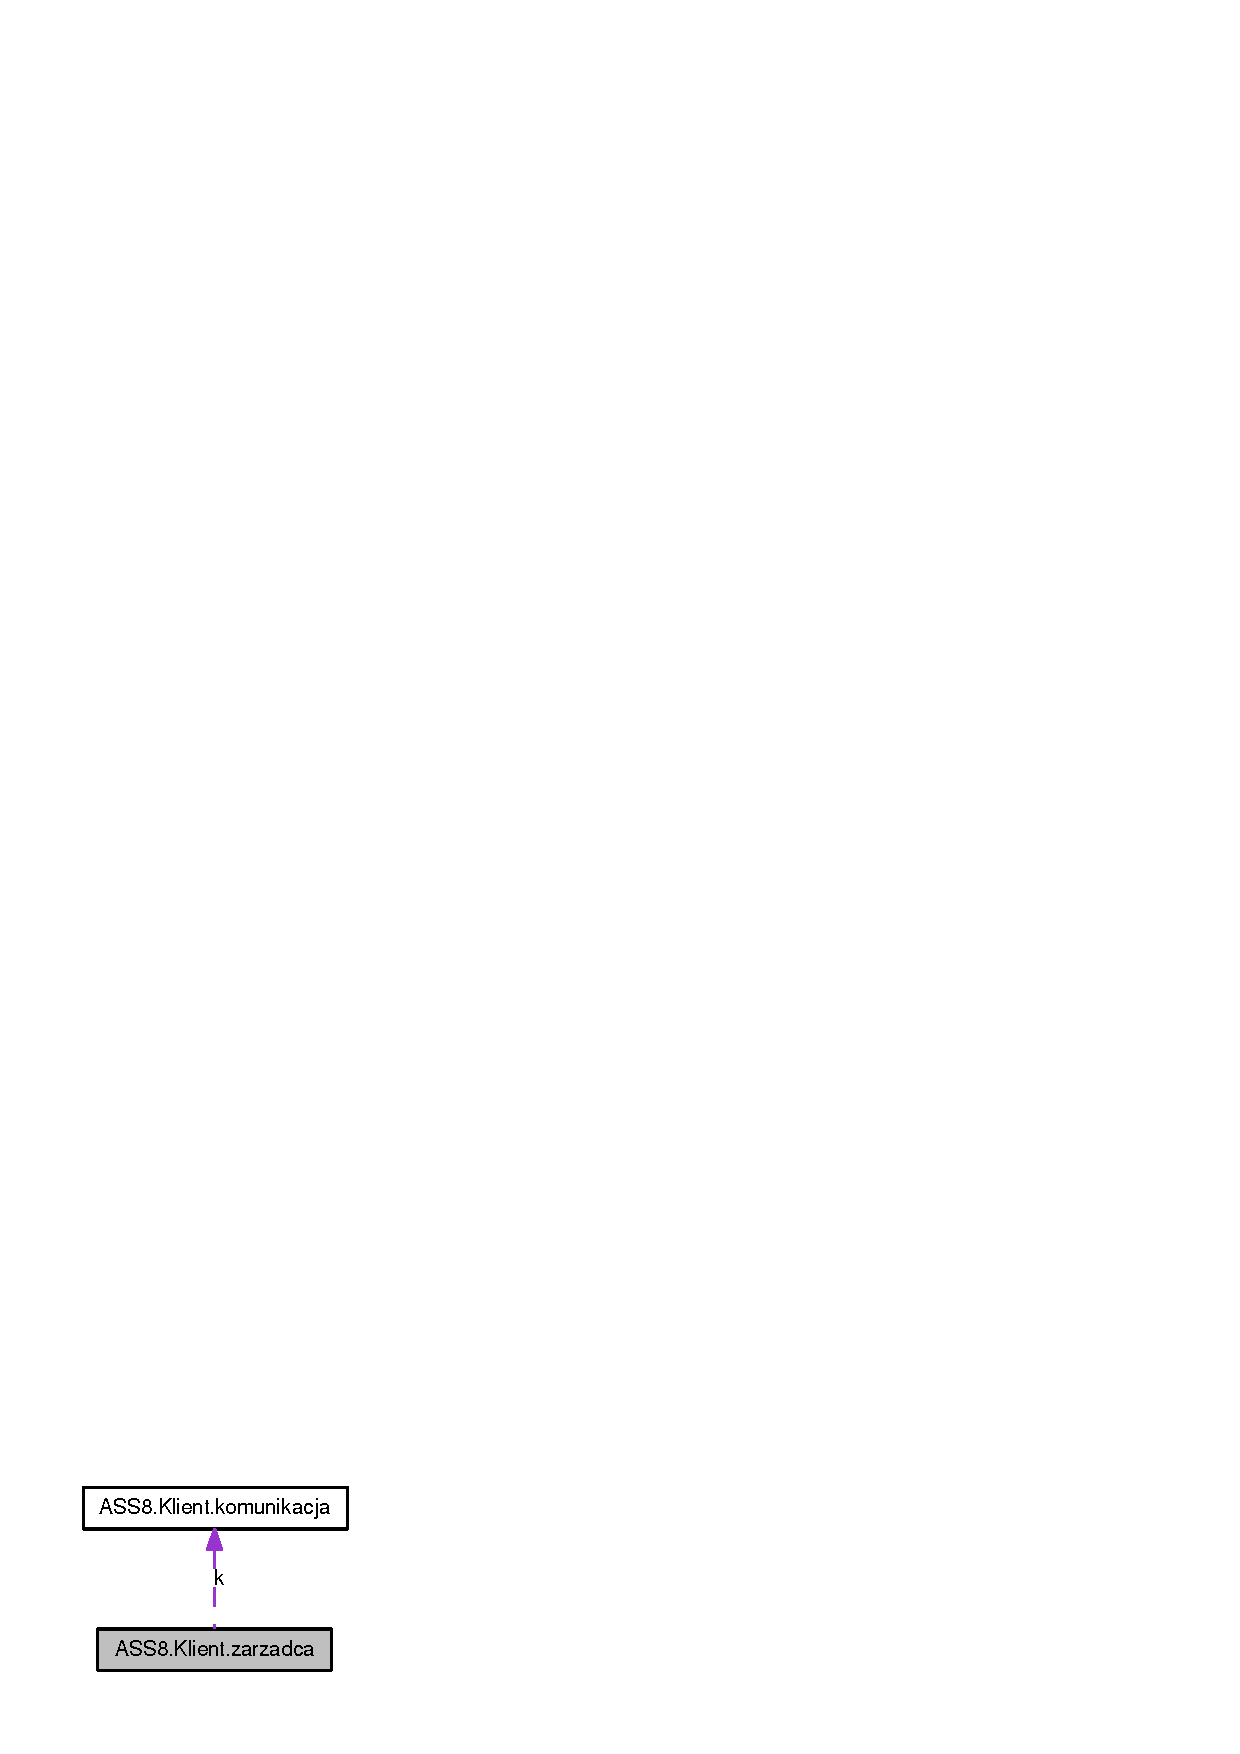
\includegraphics[width=170pt]{d3/dd5/a00215}
\end{center}
\end{figure}
\subsection*{Metody publiczne}
\begin{CompactItemize}
\item 
void \hyperlink{a00037_facd9f376d18bedf9eb790ea68e23cf2}{zmianaKontroli} (int kontrola)
\begin{CompactList}\small\item\em Zmienia kontroli błędów (gdzie ma być wypisywany komunikat o bledach). \item\end{CompactList}\item 
\hyperlink{a00037_fefaf155f21b7d7cafd855f1c3fdb21d}{zarzadca} (\hyperlink{a00013}{komunikacja} kom, NotifyIcon ni, int b, string fol)
\begin{CompactList}\small\item\em Konstruktor klasy, inicjalizuje wszystkie zmienne oraz tworzy katalog użytkownika jeżeli nie istnieje. \item\end{CompactList}\item 
void \hyperlink{a00037_0b7572681d52b2aff3d3b300639e66b9}{zapiszInfoPlikow} ()
\begin{CompactList}\small\item\em Zapisuje do pliku konfiguracyjnego wszystkie \hyperlink{a00017}{pliki} znajdujące się w katalogu. \item\end{CompactList}\item 
void \hyperlink{a00037_23c6a981e5d8340c7207a7cbbd5d710e}{szukajZmian} ()
\begin{CompactList}\small\item\em Funkcja sprawdza jakie zmieny nastąpiły na dysku lub serwerze i w zależności od tego jakie \hyperlink{a00017}{pliki} się pojawiły podejmuje odpowiednią akcję. \item\end{CompactList}\end{CompactItemize}
\subsection*{Atrybuty publiczne}
\begin{CompactItemize}
\item 
string \hyperlink{a00037_e91fc8825b76e32fee5742c3454aaee0}{folder}
\begin{CompactList}\small\item\em Zmienna przechowuje folder użytkownika. \item\end{CompactList}\item 
Mutex \hyperlink{a00037_1ff0a9cb09ec0877a4411793dc5683f7}{folderMutex}
\item 
Mutex \hyperlink{a00037_92cb338fa86bdf0e8f952202ffa362ca}{mutex}
\end{CompactItemize}
\subsection*{Właściwości}
\begin{CompactItemize}
\item 
\hyperlink{a00013}{komunikacja} \hyperlink{a00037_a13c5d1237dd3ac1519ea0225757fce5}{kom}\hspace{0.3cm}{\tt  \mbox{[}set\mbox{]}}
\end{CompactItemize}
\subsection*{Metody prywatne}
\begin{CompactItemize}
\item 
void \hyperlink{a00037_d94f9cb612f02daf94e197aae7a25c4d}{wyswietlBlad} (string str)
\begin{CompactList}\small\item\em Wyświetla błąd w trayu. \item\end{CompactList}\item 
void \hyperlink{a00037_b543bc78feea7f86bace90f920f17511}{zapiszBlad} (string str)
\begin{CompactList}\small\item\em Zapisuje błąd do pliku. \item\end{CompactList}\item 
List$<$ \hyperlink{a00018}{plikInfo} $>$ \hyperlink{a00037_55b06ff6e65c5b3668ddd5e299528beb}{sprawdzRoznicaDownload} (List$<$ \hyperlink{a00018}{plikInfo} $>$ serwer, \hyperlink{a00017}{pliki} plik, \hyperlink{a00017}{pliki} katalog)
\begin{CompactList}\small\item\em Sprawdza które \hyperlink{a00017}{pliki} należy ściągnąć z serwera. \item\end{CompactList}\item 
List$<$ \hyperlink{a00020}{pojedynczyPlik} $>$ \hyperlink{a00037_8f5d03264bce3d51a12bbda9b4fd464d}{sprawdzRoznicaUpload} (List$<$ \hyperlink{a00018}{plikInfo} $>$ serwer, \hyperlink{a00017}{pliki} plik, \hyperlink{a00017}{pliki} katalog)
\begin{CompactList}\small\item\em Sprawdza które \hyperlink{a00017}{pliki} należy wysłać na serwer. \item\end{CompactList}\item 
List$<$ \hyperlink{a00020}{pojedynczyPlik} $>$ \hyperlink{a00037_a1c9556bf17ca6296a65c8ce4c2e345a}{sprawdzRoznicaUsunKatalog} (List$<$ \hyperlink{a00018}{plikInfo} $>$ serwer, \hyperlink{a00017}{pliki} plik, \hyperlink{a00017}{pliki} katalog)
\begin{CompactList}\small\item\em Sprawdza które \hyperlink{a00017}{pliki} należy usunąć z dysku. \item\end{CompactList}\item 
List$<$ \hyperlink{a00020}{pojedynczyPlik} $>$ \hyperlink{a00037_e15914ff83794a5f6fb1e848c7640900}{sprawdzRoznicaUsunSerwer} (List$<$ \hyperlink{a00018}{plikInfo} $>$ serwer, \hyperlink{a00017}{pliki} plik, \hyperlink{a00017}{pliki} katalog)
\begin{CompactList}\small\item\em Sprawdza które \hyperlink{a00017}{pliki} należy usunąć z serwera. \item\end{CompactList}\item 
void \hyperlink{a00037_c6dbb2e2034a04a7abf666b24b419b6b}{odbierzPliki} (List$<$ \hyperlink{a00018}{plikInfo} $>$ plikiDoSciagniecia)
\begin{CompactList}\small\item\em Odbiera \hyperlink{a00017}{pliki} z serwera. \item\end{CompactList}\item 
void \hyperlink{a00037_ecff337c51d7c6aec79286ad97745b47}{wyslijPlik} (List$<$ \hyperlink{a00020}{pojedynczyPlik} $>$ plikiDoWyslania)
\begin{CompactList}\small\item\em Wysyła \hyperlink{a00017}{pliki} na serwer. \item\end{CompactList}\item 
\hyperlink{a00017}{pliki} \hyperlink{a00037_2806aca42bed01f5fefc1bda76b1f250}{plikiZapisane} ()
\begin{CompactList}\small\item\em Pobiera listę plików z pliku konfiguracyjnego. \item\end{CompactList}\item 
string \hyperlink{a00037_565af80b3fd64edae29abc5210555614}{hashPliku} (string plik)
\begin{CompactList}\small\item\em Oblicza hash pliku w MD5. \item\end{CompactList}\item 
void \hyperlink{a00037_4b2c5e502366b63f4115cecdb5873ccb}{wykasujPlik} (List$<$ \hyperlink{a00020}{pojedynczyPlik} $>$ \hyperlink{a00017}{pliki})
\begin{CompactList}\small\item\em Kasuje plik z dysku. \item\end{CompactList}\item 
void \hyperlink{a00037_0eb71b522a777a8dba01615aa58b2203}{plikiKatalog} (string katalog, \hyperlink{a00017}{pliki} lista)
\begin{CompactList}\small\item\em Zprawdza jakie \hyperlink{a00017}{pliki} są w katalogu. \item\end{CompactList}\item 
List$<$ \hyperlink{a00020}{pojedynczyPlik} $>$ \hyperlink{a00037_929f999868b8425b4b6ae6a835187e22}{sprawdzAktualizacje} (\hyperlink{a00017}{pliki} plik, \hyperlink{a00017}{pliki} katalog, List$<$ \hyperlink{a00018}{plikInfo} $>$ serwer)
\begin{CompactList}\small\item\em Sprawdza jakie są różnice pomiędzy plikami na serwerze i w katalogu. \item\end{CompactList}\item 
List$<$ \hyperlink{a00018}{plikInfo} $>$ \hyperlink{a00037_605e903992f33680e874e6685760786a}{sprawdzAktualizacje} (List$<$ \hyperlink{a00018}{plikInfo} $>$ serwer, \hyperlink{a00017}{pliki} plik, \hyperlink{a00017}{pliki} katalog)
\begin{CompactList}\small\item\em Sprawdza jakie są różnice pomiędzy plikami na serwerze i w katalogu. \item\end{CompactList}\item 
void \hyperlink{a00037_8c6fafc63cea03167c3cac60d6ebf3a3}{usunPliki} (List$<$ \hyperlink{a00020}{pojedynczyPlik} $>$ \hyperlink{a00017}{pliki})
\begin{CompactList}\small\item\em Sprawdza jakie są różnice pomiędzy plikami na serwerze i w katalogu. \item\end{CompactList}\end{CompactItemize}
\subsection*{Atrybuty prywatne}
\begin{CompactItemize}
\item 
\hyperlink{a00013}{komunikacja} \hyperlink{a00037_b7fef33c2cf29406276fbbb926338c96}{k}
\begin{CompactList}\small\item\em Zmienna przechowuje klasę do obsługi sieciowej. \item\end{CompactList}\item 
string \hyperlink{a00037_064dde1d0807e0df79bbf7b697878583}{login}
\begin{CompactList}\small\item\em Zmienna przechowuje login użytkownika. \item\end{CompactList}\item 
int \hyperlink{a00037_3d392ffd05da1da4971c8f2629be04eb}{kontrolaBledow}
\item 
XmlSerializerNamespaces \hyperlink{a00037_ade6b1a7122cb3a1f7d719376694dd0e}{names}
\item 
NotifyIcon \hyperlink{a00037_7c6e834f62b4eb8c8138b736497c9a56}{notify}
\end{CompactItemize}


\subsection{Opis szczegółowy}
Klasa zarządzająca połączeniem i wszystkimi operacjami z plikami. 



Definicja w linii 15 pliku zarzadca.cs.

\subsection{Dokumentacja konstruktora i destruktora}
\hypertarget{a00037_fefaf155f21b7d7cafd855f1c3fdb21d}{
\index{ASS8::Klient::zarzadca@{ASS8::Klient::zarzadca}!zarzadca@{zarzadca}}
\index{zarzadca@{zarzadca}!ASS8::Klient::zarzadca@{ASS8::Klient::zarzadca}}
\subsubsection[{zarzadca}]{\setlength{\rightskip}{0pt plus 5cm}ASS8.Klient.zarzadca.zarzadca ({\bf komunikacja} {\em kom}, \/  NotifyIcon {\em ni}, \/  int {\em b}, \/  string {\em fol})}}
\label{d1/dc6/a00037_fefaf155f21b7d7cafd855f1c3fdb21d}


Konstruktor klasy, inicjalizuje wszystkie zmienne oraz tworzy katalog użytkownika jeżeli nie istnieje. 

\begin{Desc}
\item[Parametry:]
\begin{description}
\item[{\em kom}]Zmienna do obsługi sieciowej\item[{\em ni}]Zmienna ikony traya\item[{\em b}]Zmienna z obsługą błędów\item[{\em fol}]Folder użytkownika\end{description}
\end{Desc}


Definicja w linii 49 pliku zarzadca.cs.

\subsection{Dokumentacja funkcji składowych}
\hypertarget{a00037_565af80b3fd64edae29abc5210555614}{
\index{ASS8::Klient::zarzadca@{ASS8::Klient::zarzadca}!hashPliku@{hashPliku}}
\index{hashPliku@{hashPliku}!ASS8::Klient::zarzadca@{ASS8::Klient::zarzadca}}
\subsubsection[{hashPliku}]{\setlength{\rightskip}{0pt plus 5cm}string ASS8.Klient.zarzadca.hashPliku (string {\em plik})\hspace{0.3cm}{\tt  \mbox{[}private\mbox{]}}}}
\label{d1/dc6/a00037_565af80b3fd64edae29abc5210555614}


Oblicza hash pliku w MD5. 

\begin{Desc}
\item[Parametry:]
\begin{description}
\item[{\em plik}]Nazwa pliku do zakodowania\end{description}
\end{Desc}
\begin{Desc}
\item[Zwraca:]Hash pliku\end{Desc}


Definicja w linii 259 pliku zarzadca.cs.\hypertarget{a00037_c6dbb2e2034a04a7abf666b24b419b6b}{
\index{ASS8::Klient::zarzadca@{ASS8::Klient::zarzadca}!odbierzPliki@{odbierzPliki}}
\index{odbierzPliki@{odbierzPliki}!ASS8::Klient::zarzadca@{ASS8::Klient::zarzadca}}
\subsubsection[{odbierzPliki}]{\setlength{\rightskip}{0pt plus 5cm}void ASS8.Klient.zarzadca.odbierzPliki (List$<$ {\bf plikInfo} $>$ {\em plikiDoSciagniecia})\hspace{0.3cm}{\tt  \mbox{[}private\mbox{]}}}}
\label{d1/dc6/a00037_c6dbb2e2034a04a7abf666b24b419b6b}


Odbiera \hyperlink{a00017}{pliki} z serwera. 

\begin{Desc}
\item[Parametry:]
\begin{description}
\item[{\em plikiDoSciagniecia}]Lista plików do ściągnięcia\end{description}
\end{Desc}


Definicja w linii 185 pliku zarzadca.cs.\hypertarget{a00037_0eb71b522a777a8dba01615aa58b2203}{
\index{ASS8::Klient::zarzadca@{ASS8::Klient::zarzadca}!plikiKatalog@{plikiKatalog}}
\index{plikiKatalog@{plikiKatalog}!ASS8::Klient::zarzadca@{ASS8::Klient::zarzadca}}
\subsubsection[{plikiKatalog}]{\setlength{\rightskip}{0pt plus 5cm}void ASS8.Klient.zarzadca.plikiKatalog (string {\em katalog}, \/  {\bf pliki} {\em lista})\hspace{0.3cm}{\tt  \mbox{[}private\mbox{]}}}}
\label{d1/dc6/a00037_0eb71b522a777a8dba01615aa58b2203}


Zprawdza jakie \hyperlink{a00017}{pliki} są w katalogu. 

\begin{Desc}
\item[Parametry:]
\begin{description}
\item[{\em katalog}]Katalog w którym ma sprawdzać\item[{\em lista}]Lista plików jakie się znajdują w katalogu\end{description}
\end{Desc}


Definicja w linii 299 pliku zarzadca.cs.\hypertarget{a00037_2806aca42bed01f5fefc1bda76b1f250}{
\index{ASS8::Klient::zarzadca@{ASS8::Klient::zarzadca}!plikiZapisane@{plikiZapisane}}
\index{plikiZapisane@{plikiZapisane}!ASS8::Klient::zarzadca@{ASS8::Klient::zarzadca}}
\subsubsection[{plikiZapisane}]{\setlength{\rightskip}{0pt plus 5cm}{\bf pliki} ASS8.Klient.zarzadca.plikiZapisane ()\hspace{0.3cm}{\tt  \mbox{[}private\mbox{]}}}}
\label{d1/dc6/a00037_2806aca42bed01f5fefc1bda76b1f250}


Pobiera listę plików z pliku konfiguracyjnego. 

\begin{Desc}
\item[Zwraca:]Zmienna przechowująca wszystkie \hyperlink{a00017}{pliki} zapisane\end{Desc}


Definicja w linii 232 pliku zarzadca.cs.\hypertarget{a00037_605e903992f33680e874e6685760786a}{
\index{ASS8::Klient::zarzadca@{ASS8::Klient::zarzadca}!sprawdzAktualizacje@{sprawdzAktualizacje}}
\index{sprawdzAktualizacje@{sprawdzAktualizacje}!ASS8::Klient::zarzadca@{ASS8::Klient::zarzadca}}
\subsubsection[{sprawdzAktualizacje}]{\setlength{\rightskip}{0pt plus 5cm}List$<${\bf plikInfo}$>$ ASS8.Klient.zarzadca.sprawdzAktualizacje (List$<$ {\bf plikInfo} $>$ {\em serwer}, \/  {\bf pliki} {\em plik}, \/  {\bf pliki} {\em katalog})\hspace{0.3cm}{\tt  \mbox{[}private\mbox{]}}}}
\label{d1/dc6/a00037_605e903992f33680e874e6685760786a}


Sprawdza jakie są różnice pomiędzy plikami na serwerze i w katalogu. 

\begin{Desc}
\item[Parametry:]
\begin{description}
\item[{\em plik}]Lista plikow w pliku konfiguracyjnym\item[{\em katalog}]Lista plików w katalogu\item[{\em serwer}]Lista plików na serwerze\end{description}
\end{Desc}
\begin{Desc}
\item[Zwraca:]Lista plików do aktualizacji\end{Desc}


Definicja w linii 417 pliku zarzadca.cs.\hypertarget{a00037_929f999868b8425b4b6ae6a835187e22}{
\index{ASS8::Klient::zarzadca@{ASS8::Klient::zarzadca}!sprawdzAktualizacje@{sprawdzAktualizacje}}
\index{sprawdzAktualizacje@{sprawdzAktualizacje}!ASS8::Klient::zarzadca@{ASS8::Klient::zarzadca}}
\subsubsection[{sprawdzAktualizacje}]{\setlength{\rightskip}{0pt plus 5cm}List$<${\bf pojedynczyPlik}$>$ ASS8.Klient.zarzadca.sprawdzAktualizacje ({\bf pliki} {\em plik}, \/  {\bf pliki} {\em katalog}, \/  List$<$ {\bf plikInfo} $>$ {\em serwer})\hspace{0.3cm}{\tt  \mbox{[}private\mbox{]}}}}
\label{d1/dc6/a00037_929f999868b8425b4b6ae6a835187e22}


Sprawdza jakie są różnice pomiędzy plikami na serwerze i w katalogu. 

\begin{Desc}
\item[Parametry:]
\begin{description}
\item[{\em plik}]Lista plikow w pliku konfiguracyjnym\item[{\em katalog}]Lista plików w katalogu\item[{\em serwer}]Lista plików na serwerze\end{description}
\end{Desc}
\begin{Desc}
\item[Zwraca:]Lista plików do aktualizacji\end{Desc}


Definicja w linii 393 pliku zarzadca.cs.\hypertarget{a00037_55b06ff6e65c5b3668ddd5e299528beb}{
\index{ASS8::Klient::zarzadca@{ASS8::Klient::zarzadca}!sprawdzRoznicaDownload@{sprawdzRoznicaDownload}}
\index{sprawdzRoznicaDownload@{sprawdzRoznicaDownload}!ASS8::Klient::zarzadca@{ASS8::Klient::zarzadca}}
\subsubsection[{sprawdzRoznicaDownload}]{\setlength{\rightskip}{0pt plus 5cm}List$<${\bf plikInfo}$>$ ASS8.Klient.zarzadca.sprawdzRoznicaDownload (List$<$ {\bf plikInfo} $>$ {\em serwer}, \/  {\bf pliki} {\em plik}, \/  {\bf pliki} {\em katalog})\hspace{0.3cm}{\tt  \mbox{[}private\mbox{]}}}}
\label{d1/dc6/a00037_55b06ff6e65c5b3668ddd5e299528beb}


Sprawdza które \hyperlink{a00017}{pliki} należy ściągnąć z serwera. 

\begin{Desc}
\item[Parametry:]
\begin{description}
\item[{\em serwer}]Pliki na serwerze\item[{\em plik}]Pliki zapisane w pliku konfiguracyjnym\item[{\em katalog}]Pliki w katalogu\end{description}
\end{Desc}
\begin{Desc}
\item[Zwraca:]Lista plików do ściągnięcia\end{Desc}


Definicja w linii 97 pliku zarzadca.cs.\hypertarget{a00037_8f5d03264bce3d51a12bbda9b4fd464d}{
\index{ASS8::Klient::zarzadca@{ASS8::Klient::zarzadca}!sprawdzRoznicaUpload@{sprawdzRoznicaUpload}}
\index{sprawdzRoznicaUpload@{sprawdzRoznicaUpload}!ASS8::Klient::zarzadca@{ASS8::Klient::zarzadca}}
\subsubsection[{sprawdzRoznicaUpload}]{\setlength{\rightskip}{0pt plus 5cm}List$<${\bf pojedynczyPlik}$>$ ASS8.Klient.zarzadca.sprawdzRoznicaUpload (List$<$ {\bf plikInfo} $>$ {\em serwer}, \/  {\bf pliki} {\em plik}, \/  {\bf pliki} {\em katalog})\hspace{0.3cm}{\tt  \mbox{[}private\mbox{]}}}}
\label{d1/dc6/a00037_8f5d03264bce3d51a12bbda9b4fd464d}


Sprawdza które \hyperlink{a00017}{pliki} należy wysłać na serwer. 

\begin{Desc}
\item[Parametry:]
\begin{description}
\item[{\em serwer}]Pliki na serwerze\item[{\em plik}]Pliki zapisane w pliku konfiguracyjnym\item[{\em katalog}]Pliki w katalogu\end{description}
\end{Desc}
\begin{Desc}
\item[Zwraca:]Lista plików wysłania\end{Desc}


Definicja w linii 117 pliku zarzadca.cs.\hypertarget{a00037_a1c9556bf17ca6296a65c8ce4c2e345a}{
\index{ASS8::Klient::zarzadca@{ASS8::Klient::zarzadca}!sprawdzRoznicaUsunKatalog@{sprawdzRoznicaUsunKatalog}}
\index{sprawdzRoznicaUsunKatalog@{sprawdzRoznicaUsunKatalog}!ASS8::Klient::zarzadca@{ASS8::Klient::zarzadca}}
\subsubsection[{sprawdzRoznicaUsunKatalog}]{\setlength{\rightskip}{0pt plus 5cm}List$<${\bf pojedynczyPlik}$>$ ASS8.Klient.zarzadca.sprawdzRoznicaUsunKatalog (List$<$ {\bf plikInfo} $>$ {\em serwer}, \/  {\bf pliki} {\em plik}, \/  {\bf pliki} {\em katalog})\hspace{0.3cm}{\tt  \mbox{[}private\mbox{]}}}}
\label{d1/dc6/a00037_a1c9556bf17ca6296a65c8ce4c2e345a}


Sprawdza które \hyperlink{a00017}{pliki} należy usunąć z dysku. 

\begin{Desc}
\item[Parametry:]
\begin{description}
\item[{\em serwer}]Pliki na serwerze\item[{\em plik}]Pliki zapisane w pliku konfiguracyjnym\item[{\em katalog}]Pliki w katalogu\end{description}
\end{Desc}
\begin{Desc}
\item[Zwraca:]Lista plików do usunięcia\end{Desc}


Definicja w linii 137 pliku zarzadca.cs.\hypertarget{a00037_e15914ff83794a5f6fb1e848c7640900}{
\index{ASS8::Klient::zarzadca@{ASS8::Klient::zarzadca}!sprawdzRoznicaUsunSerwer@{sprawdzRoznicaUsunSerwer}}
\index{sprawdzRoznicaUsunSerwer@{sprawdzRoznicaUsunSerwer}!ASS8::Klient::zarzadca@{ASS8::Klient::zarzadca}}
\subsubsection[{sprawdzRoznicaUsunSerwer}]{\setlength{\rightskip}{0pt plus 5cm}List$<${\bf pojedynczyPlik}$>$ ASS8.Klient.zarzadca.sprawdzRoznicaUsunSerwer (List$<$ {\bf plikInfo} $>$ {\em serwer}, \/  {\bf pliki} {\em plik}, \/  {\bf pliki} {\em katalog})\hspace{0.3cm}{\tt  \mbox{[}private\mbox{]}}}}
\label{d1/dc6/a00037_e15914ff83794a5f6fb1e848c7640900}


Sprawdza które \hyperlink{a00017}{pliki} należy usunąć z serwera. 

\begin{Desc}
\item[Parametry:]
\begin{description}
\item[{\em serwer}]Pliki na serwerze\item[{\em plik}]Pliki zapisane w pliku konfiguracyjnym\item[{\em katalog}]Pliki w katalogu\end{description}
\end{Desc}
\begin{Desc}
\item[Zwraca:]Lista plików do usunięcia\end{Desc}


Definicja w linii 156 pliku zarzadca.cs.\hypertarget{a00037_23c6a981e5d8340c7207a7cbbd5d710e}{
\index{ASS8::Klient::zarzadca@{ASS8::Klient::zarzadca}!szukajZmian@{szukajZmian}}
\index{szukajZmian@{szukajZmian}!ASS8::Klient::zarzadca@{ASS8::Klient::zarzadca}}
\subsubsection[{szukajZmian}]{\setlength{\rightskip}{0pt plus 5cm}void ASS8.Klient.zarzadca.szukajZmian ()}}
\label{d1/dc6/a00037_23c6a981e5d8340c7207a7cbbd5d710e}


Funkcja sprawdza jakie zmieny nastąpiły na dysku lub serwerze i w zależności od tego jakie \hyperlink{a00017}{pliki} się pojawiły podejmuje odpowiednią akcję. 



Definicja w linii 326 pliku zarzadca.cs.

Here is the caller graph for this function:\nopagebreak
\begin{figure}[H]
\begin{center}
\leavevmode
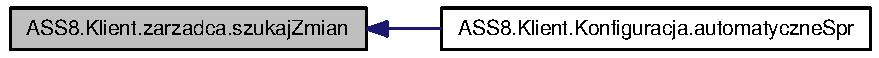
\includegraphics[width=229pt]{d1/dc6/a00037_23c6a981e5d8340c7207a7cbbd5d710e_icgraph}
\end{center}
\end{figure}
\hypertarget{a00037_8c6fafc63cea03167c3cac60d6ebf3a3}{
\index{ASS8::Klient::zarzadca@{ASS8::Klient::zarzadca}!usunPliki@{usunPliki}}
\index{usunPliki@{usunPliki}!ASS8::Klient::zarzadca@{ASS8::Klient::zarzadca}}
\subsubsection[{usunPliki}]{\setlength{\rightskip}{0pt plus 5cm}void ASS8.Klient.zarzadca.usunPliki (List$<$ {\bf pojedynczyPlik} $>$ {\em pliki})\hspace{0.3cm}{\tt  \mbox{[}private\mbox{]}}}}
\label{d1/dc6/a00037_8c6fafc63cea03167c3cac60d6ebf3a3}


Sprawdza jakie są różnice pomiędzy plikami na serwerze i w katalogu. 

\begin{Desc}
\item[Parametry:]
\begin{description}
\item[{\em plik}]Lista plikow w pliku konfiguracyjnym\item[{\em katalog}]Lista plików w katalogu\item[{\em serwer}]Lista plików na serwerze\end{description}
\end{Desc}
\begin{Desc}
\item[Zwraca:]Lista plików do aktualizacji\end{Desc}


Definicja w linii 441 pliku zarzadca.cs.\hypertarget{a00037_4b2c5e502366b63f4115cecdb5873ccb}{
\index{ASS8::Klient::zarzadca@{ASS8::Klient::zarzadca}!wykasujPlik@{wykasujPlik}}
\index{wykasujPlik@{wykasujPlik}!ASS8::Klient::zarzadca@{ASS8::Klient::zarzadca}}
\subsubsection[{wykasujPlik}]{\setlength{\rightskip}{0pt plus 5cm}void ASS8.Klient.zarzadca.wykasujPlik (List$<$ {\bf pojedynczyPlik} $>$ {\em pliki})\hspace{0.3cm}{\tt  \mbox{[}private\mbox{]}}}}
\label{d1/dc6/a00037_4b2c5e502366b63f4115cecdb5873ccb}


Kasuje plik z dysku. 

\begin{Desc}
\item[Parametry:]
\begin{description}
\item[{\em \hyperlink{a00017}{pliki}}]Lista plików do usunięcia\end{description}
\end{Desc}


Definicja w linii 275 pliku zarzadca.cs.\hypertarget{a00037_ecff337c51d7c6aec79286ad97745b47}{
\index{ASS8::Klient::zarzadca@{ASS8::Klient::zarzadca}!wyslijPlik@{wyslijPlik}}
\index{wyslijPlik@{wyslijPlik}!ASS8::Klient::zarzadca@{ASS8::Klient::zarzadca}}
\subsubsection[{wyslijPlik}]{\setlength{\rightskip}{0pt plus 5cm}void ASS8.Klient.zarzadca.wyslijPlik (List$<$ {\bf pojedynczyPlik} $>$ {\em plikiDoWyslania})\hspace{0.3cm}{\tt  \mbox{[}private\mbox{]}}}}
\label{d1/dc6/a00037_ecff337c51d7c6aec79286ad97745b47}


Wysyła \hyperlink{a00017}{pliki} na serwer. 

\begin{Desc}
\item[Parametry:]
\begin{description}
\item[{\em plikiDoWyslania}]Lista plików do wysłania\end{description}
\end{Desc}


Definicja w linii 208 pliku zarzadca.cs.\hypertarget{a00037_d94f9cb612f02daf94e197aae7a25c4d}{
\index{ASS8::Klient::zarzadca@{ASS8::Klient::zarzadca}!wyswietlBlad@{wyswietlBlad}}
\index{wyswietlBlad@{wyswietlBlad}!ASS8::Klient::zarzadca@{ASS8::Klient::zarzadca}}
\subsubsection[{wyswietlBlad}]{\setlength{\rightskip}{0pt plus 5cm}void ASS8.Klient.zarzadca.wyswietlBlad (string {\em str})\hspace{0.3cm}{\tt  \mbox{[}private\mbox{]}}}}
\label{d1/dc6/a00037_d94f9cb612f02daf94e197aae7a25c4d}


Wyświetla błąd w trayu. 

\begin{Desc}
\item[Parametry:]
\begin{description}
\item[{\em str}]Wiadomość do wyświetlenia\end{description}
\end{Desc}


Definicja w linii 76 pliku zarzadca.cs.\hypertarget{a00037_b543bc78feea7f86bace90f920f17511}{
\index{ASS8::Klient::zarzadca@{ASS8::Klient::zarzadca}!zapiszBlad@{zapiszBlad}}
\index{zapiszBlad@{zapiszBlad}!ASS8::Klient::zarzadca@{ASS8::Klient::zarzadca}}
\subsubsection[{zapiszBlad}]{\setlength{\rightskip}{0pt plus 5cm}void ASS8.Klient.zarzadca.zapiszBlad (string {\em str})\hspace{0.3cm}{\tt  \mbox{[}private\mbox{]}}}}
\label{d1/dc6/a00037_b543bc78feea7f86bace90f920f17511}


Zapisuje błąd do pliku. 

\begin{Desc}
\item[Parametry:]
\begin{description}
\item[{\em str}]Wiadomość do zapisywania\end{description}
\end{Desc}


Definicja w linii 83 pliku zarzadca.cs.\hypertarget{a00037_0b7572681d52b2aff3d3b300639e66b9}{
\index{ASS8::Klient::zarzadca@{ASS8::Klient::zarzadca}!zapiszInfoPlikow@{zapiszInfoPlikow}}
\index{zapiszInfoPlikow@{zapiszInfoPlikow}!ASS8::Klient::zarzadca@{ASS8::Klient::zarzadca}}
\subsubsection[{zapiszInfoPlikow}]{\setlength{\rightskip}{0pt plus 5cm}void ASS8.Klient.zarzadca.zapiszInfoPlikow ()}}
\label{d1/dc6/a00037_0b7572681d52b2aff3d3b300639e66b9}


Zapisuje do pliku konfiguracyjnego wszystkie \hyperlink{a00017}{pliki} znajdujące się w katalogu. 



Definicja w linii 172 pliku zarzadca.cs.\hypertarget{a00037_facd9f376d18bedf9eb790ea68e23cf2}{
\index{ASS8::Klient::zarzadca@{ASS8::Klient::zarzadca}!zmianaKontroli@{zmianaKontroli}}
\index{zmianaKontroli@{zmianaKontroli}!ASS8::Klient::zarzadca@{ASS8::Klient::zarzadca}}
\subsubsection[{zmianaKontroli}]{\setlength{\rightskip}{0pt plus 5cm}void ASS8.Klient.zarzadca.zmianaKontroli (int {\em kontrola})}}
\label{d1/dc6/a00037_facd9f376d18bedf9eb790ea68e23cf2}


Zmienia kontroli błędów (gdzie ma być wypisywany komunikat o bledach). 

\begin{Desc}
\item[Parametry:]
\begin{description}
\item[{\em kontrola}]Zmienna określająca typ obsługi błędów\end{description}
\end{Desc}


Definicja w linii 38 pliku zarzadca.cs.

Here is the caller graph for this function:\nopagebreak
\begin{figure}[H]
\begin{center}
\leavevmode
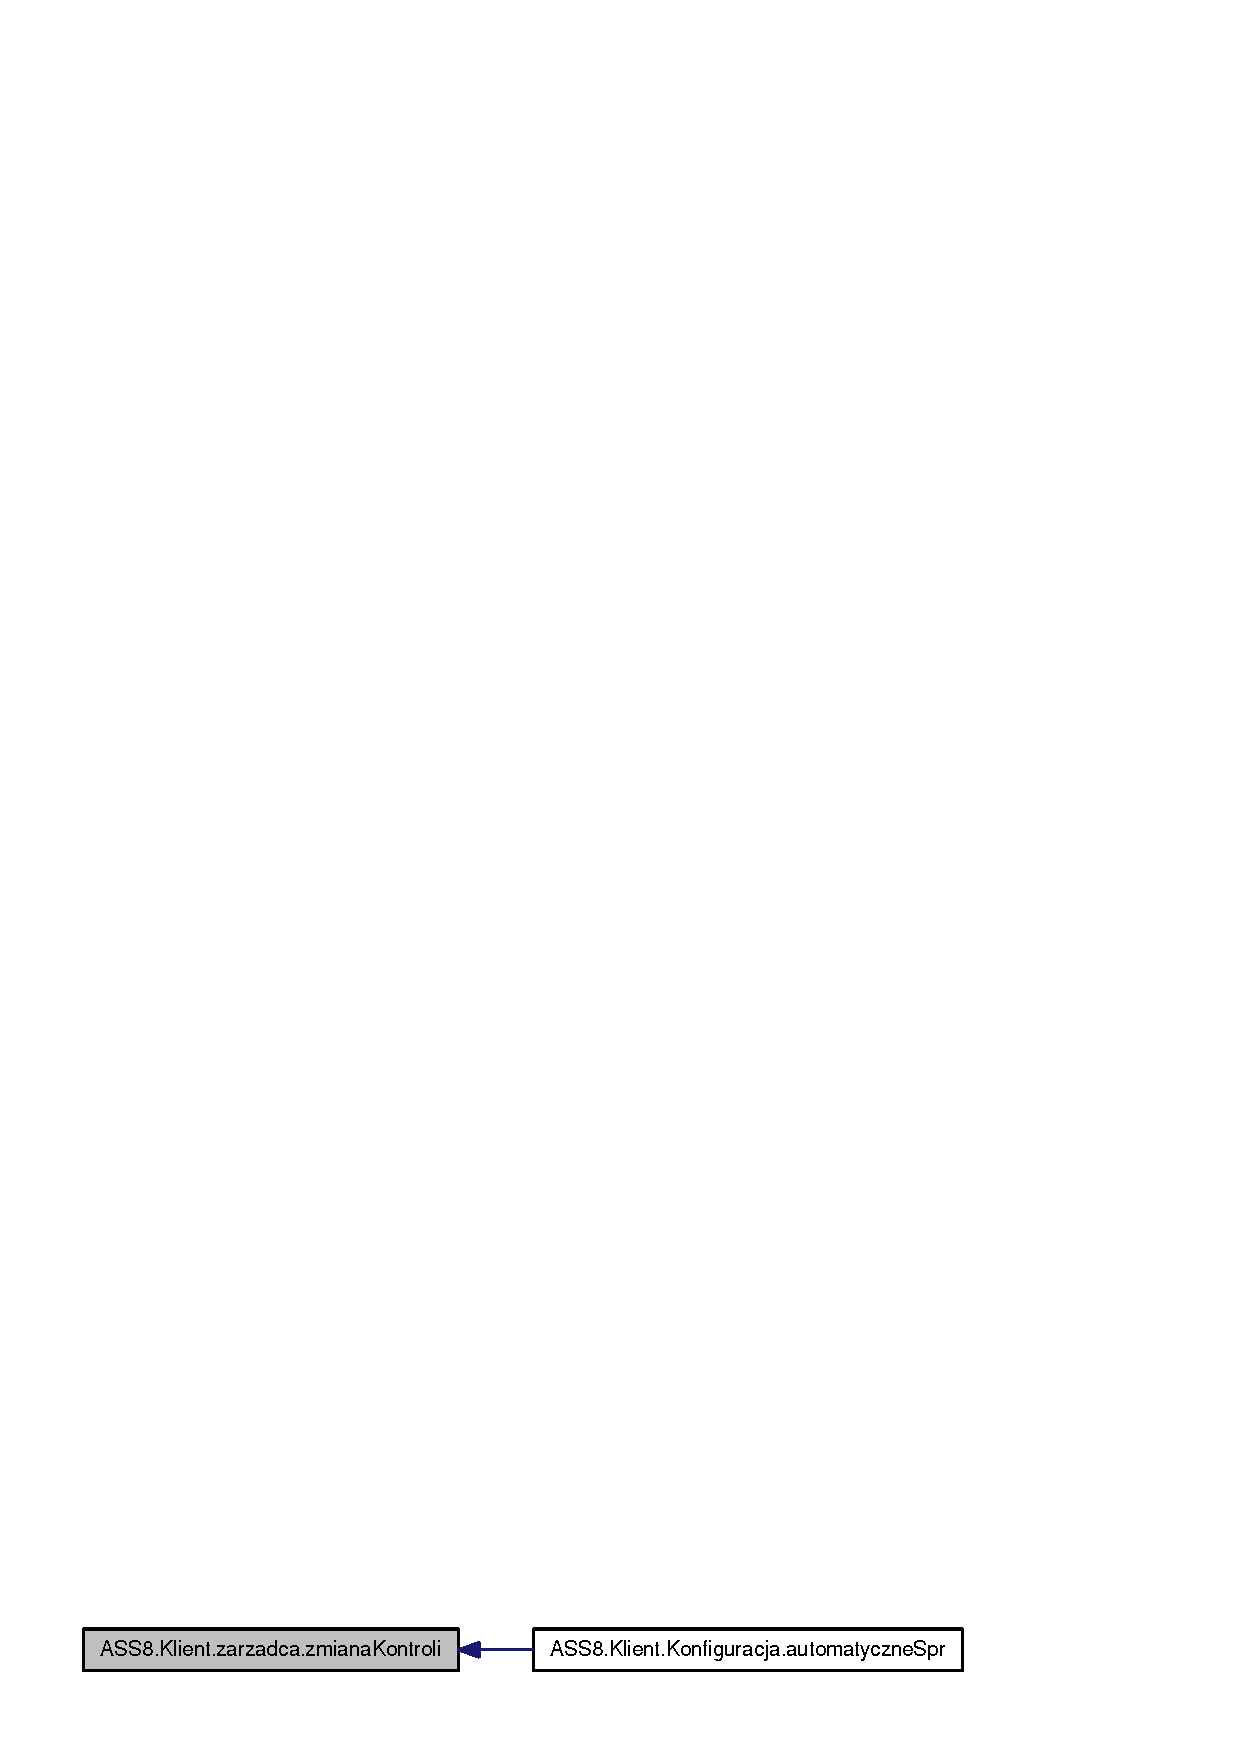
\includegraphics[width=233pt]{d1/dc6/a00037_facd9f376d18bedf9eb790ea68e23cf2_icgraph}
\end{center}
\end{figure}


\subsection{Dokumentacja atrybutów składowych}
\hypertarget{a00037_e91fc8825b76e32fee5742c3454aaee0}{
\index{ASS8::Klient::zarzadca@{ASS8::Klient::zarzadca}!folder@{folder}}
\index{folder@{folder}!ASS8::Klient::zarzadca@{ASS8::Klient::zarzadca}}
\subsubsection[{folder}]{\setlength{\rightskip}{0pt plus 5cm}string {\bf ASS8.Klient.zarzadca.folder}}}
\label{d1/dc6/a00037_e91fc8825b76e32fee5742c3454aaee0}


Zmienna przechowuje folder użytkownika. 



Definicja w linii 24 pliku zarzadca.cs.\hypertarget{a00037_1ff0a9cb09ec0877a4411793dc5683f7}{
\index{ASS8::Klient::zarzadca@{ASS8::Klient::zarzadca}!folderMutex@{folderMutex}}
\index{folderMutex@{folderMutex}!ASS8::Klient::zarzadca@{ASS8::Klient::zarzadca}}
\subsubsection[{folderMutex}]{\setlength{\rightskip}{0pt plus 5cm}Mutex {\bf ASS8.Klient.zarzadca.folderMutex}}}
\label{d1/dc6/a00037_1ff0a9cb09ec0877a4411793dc5683f7}




Definicja w linii 30 pliku zarzadca.cs.\hypertarget{a00037_b7fef33c2cf29406276fbbb926338c96}{
\index{ASS8::Klient::zarzadca@{ASS8::Klient::zarzadca}!k@{k}}
\index{k@{k}!ASS8::Klient::zarzadca@{ASS8::Klient::zarzadca}}
\subsubsection[{k}]{\setlength{\rightskip}{0pt plus 5cm}{\bf komunikacja} {\bf ASS8.Klient.zarzadca.k}\hspace{0.3cm}{\tt  \mbox{[}private\mbox{]}}}}
\label{d1/dc6/a00037_b7fef33c2cf29406276fbbb926338c96}


Zmienna przechowuje klasę do obsługi sieciowej. 



Definicja w linii 20 pliku zarzadca.cs.\hypertarget{a00037_3d392ffd05da1da4971c8f2629be04eb}{
\index{ASS8::Klient::zarzadca@{ASS8::Klient::zarzadca}!kontrolaBledow@{kontrolaBledow}}
\index{kontrolaBledow@{kontrolaBledow}!ASS8::Klient::zarzadca@{ASS8::Klient::zarzadca}}
\subsubsection[{kontrolaBledow}]{\setlength{\rightskip}{0pt plus 5cm}int {\bf ASS8.Klient.zarzadca.kontrolaBledow}\hspace{0.3cm}{\tt  \mbox{[}private\mbox{]}}}}
\label{d1/dc6/a00037_3d392ffd05da1da4971c8f2629be04eb}




Definicja w linii 29 pliku zarzadca.cs.\hypertarget{a00037_064dde1d0807e0df79bbf7b697878583}{
\index{ASS8::Klient::zarzadca@{ASS8::Klient::zarzadca}!login@{login}}
\index{login@{login}!ASS8::Klient::zarzadca@{ASS8::Klient::zarzadca}}
\subsubsection[{login}]{\setlength{\rightskip}{0pt plus 5cm}string {\bf ASS8.Klient.zarzadca.login}\hspace{0.3cm}{\tt  \mbox{[}private\mbox{]}}}}
\label{d1/dc6/a00037_064dde1d0807e0df79bbf7b697878583}


Zmienna przechowuje login użytkownika. 



Definicja w linii 28 pliku zarzadca.cs.\hypertarget{a00037_92cb338fa86bdf0e8f952202ffa362ca}{
\index{ASS8::Klient::zarzadca@{ASS8::Klient::zarzadca}!mutex@{mutex}}
\index{mutex@{mutex}!ASS8::Klient::zarzadca@{ASS8::Klient::zarzadca}}
\subsubsection[{mutex}]{\setlength{\rightskip}{0pt plus 5cm}Mutex {\bf ASS8.Klient.zarzadca.mutex}}}
\label{d1/dc6/a00037_92cb338fa86bdf0e8f952202ffa362ca}




Definicja w linii 31 pliku zarzadca.cs.\hypertarget{a00037_ade6b1a7122cb3a1f7d719376694dd0e}{
\index{ASS8::Klient::zarzadca@{ASS8::Klient::zarzadca}!names@{names}}
\index{names@{names}!ASS8::Klient::zarzadca@{ASS8::Klient::zarzadca}}
\subsubsection[{names}]{\setlength{\rightskip}{0pt plus 5cm}XmlSerializerNamespaces {\bf ASS8.Klient.zarzadca.names}\hspace{0.3cm}{\tt  \mbox{[}private\mbox{]}}}}
\label{d1/dc6/a00037_ade6b1a7122cb3a1f7d719376694dd0e}




Definicja w linii 32 pliku zarzadca.cs.\hypertarget{a00037_7c6e834f62b4eb8c8138b736497c9a56}{
\index{ASS8::Klient::zarzadca@{ASS8::Klient::zarzadca}!notify@{notify}}
\index{notify@{notify}!ASS8::Klient::zarzadca@{ASS8::Klient::zarzadca}}
\subsubsection[{notify}]{\setlength{\rightskip}{0pt plus 5cm}NotifyIcon {\bf ASS8.Klient.zarzadca.notify}\hspace{0.3cm}{\tt  \mbox{[}private\mbox{]}}}}
\label{d1/dc6/a00037_7c6e834f62b4eb8c8138b736497c9a56}




Definicja w linii 33 pliku zarzadca.cs.

\subsection{Dokumentacja właściwości}
\hypertarget{a00037_a13c5d1237dd3ac1519ea0225757fce5}{
\index{ASS8::Klient::zarzadca@{ASS8::Klient::zarzadca}!kom@{kom}}
\index{kom@{kom}!ASS8::Klient::zarzadca@{ASS8::Klient::zarzadca}}
\subsubsection[{kom}]{\setlength{\rightskip}{0pt plus 5cm}{\bf komunikacja} ASS8.Klient.zarzadca.kom\hspace{0.3cm}{\tt  \mbox{[}set\mbox{]}}}}
\label{d1/dc6/a00037_a13c5d1237dd3ac1519ea0225757fce5}




Definicja w linii 466 pliku zarzadca.cs.

Dokumentacja dla tej klasy została wygenerowana z pliku:\begin{CompactItemize}
\item 
\hyperlink{a00056}{zarzadca.cs}\end{CompactItemize}
